\documentclass[11pt,class=report,crop=false]{standalone}
\usepackage[screen]{../python}

\begin{document}


%====================================================================
\chapitre{Rétropropagation}
%====================================================================

\insertvideo{HveXkSWDeYQ}{partie 9.1. Principe de la rétropropagation}

\insertvideo{_AsV7EQw78I}{partie 9.2. Exemples de rétropropagation}

\insertvideo{ePjASZtPWM0}{partie 9.3. Sur-apprentissage et autres soucis}



\objectifs{La rétropropagation, c'est la descente de gradient appliquée aux réseaux de neurones. Nous allons étudier des problèmes variés et analyser les solutions produites par des réseaux de neurones.}

\index{retropropagation@rétropropagation}
\index{descente de gradient!retropropagation@rétropropagation}

%%%%%%%%%%%%%%%%%%%%%%%%%%%%%%%%%%%%%%%%%%%%%%%%%%%%%%%%%%%%%%%%%%%%%
\section{Principe de la rétropropagation}

Voici un jeu de données : des ronds bleus et des carrés rouges.
Nous souhaitons trouver un modèle simple qui caractérise ces données.

 
\begin{center}
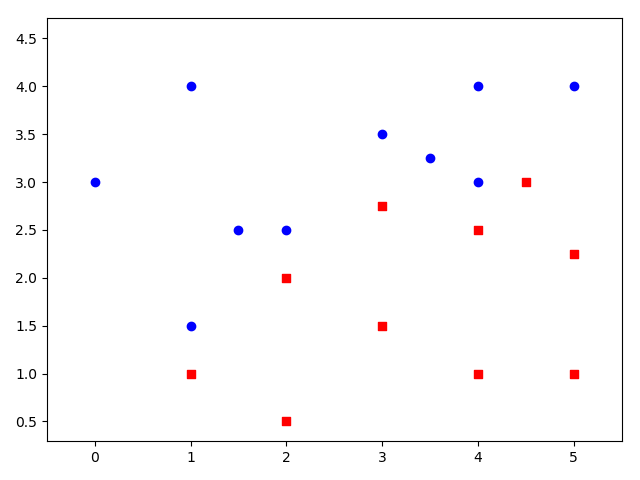
\includegraphics[scale=\myscale,scale=0.5]{figures/retro_01_a}
\end{center}

Plus exactement, nous souhaiterions pouvoir dire pour chaque point du plan s'il devrait être colorié en rouge ou bien en bleu et ceci pour des points qui ne sont pas dans les données de départ. De plus, nous voulons ne rien faire à la main, mais que la réponse soit calculée par la machine !

Nous allons revoir pas à pas l'utilisation d'un réseau de neurones pour résoudre un problème et traiterons en particulier l'exemple ci-dessus.

%--------------------------------------------------------------------
\subsection{Objectif du réseau}

\begin{itemize}
  \item Soit $\mathcal{R}$ un réseau de neurones. Celui-ci est défini par son architecture (le nombre de couches, le nombre de neurones par couche), les fonctions d'activation et l'ensemble $P = (a_1,a_2,\ldots)$ des poids de tous les neurones.
  
  \item \`A ce réseau $\mathcal{R}$ on associe une fonction $F : \Rr^n \to \Rr^p$ où $n$ est la dimension des entrées (de la première couche) et $p$ le nombre de neurones de la couche de sortie.
  Dans ce chapitre, nous supposerons qu'il n'y a qu'une seule sortie, c'est-à-dire $p=1$ et $F : \Rr^n \to \Rr$.
  
 \myfigure{0.8}{
 \tikzinput{fig_retro_04}
 } 
 
    
  \item On dispose de données $(X_i,z_i)$ (pour $i=1,\ldots,N$) où $X_i \in \Rr^n$ est une \defi{entrée} (de la forme $X=(x_1,\ldots,x_n)$) et $z_i \in \Rr$ est la \defi{sortie attendue} pour cette entrée.
  
  \item Le but est de trouver les poids du réseau afin que la fonction $F$ qui lui est associée vérifie :
  $$F(X_i) \simeq z_i \quad \text{pour tout} \quad i=1,\ldots,N.$$ 
  
  \item Pour mesurer précisément la performance de l'approximation, on définit une \defi{fonction erreur} :
  $$E = \frac{1}N \sum_{i=1}^N E_i \qquad \text{ avec } \qquad \quad E_i = \big( F(X_i) - z_i \big)^2.$$
\end{itemize}


\begin{exemple}
Nous traitons l'exemple donné en introduction.
\begin{itemize}
  \item On décide de construire le réseau le plus simple possible : avec un seul neurone. Cela correspond à séparer les points du plan selon une droite.
  On choisit la fonction d'activation $\sigma$.
  La dimension de l'entrée est $2$ et celle la sortie est $1$.
  Il y a $3$ poids $(a,b,c)$ à calculer pour terminer le paramétrage du réseau.

 \myfigure{1.5}{
 \tikzinput{fig_retro_05}
 }   

  \item Pour chaque triplet de poids $(a,b,c)$ notre réseau définit une fonction $F : \Rr^2 \to \Rr$
  qui est en fait ici :
  $$F(x,y) = \sigma(ax+by+c)$$
  avec $\sigma(t) = \frac{1}{1+e^{-t}}$.
  
  
    
  \item Nos données sont les points rouges ou bleus.
  Une entrée $X_i$ est donc constituée des coordonnées $(x_i,y_i)$ d'un point et la sortie attendue pour ce point est $z_i = 0$ (pour les points bleus) et $z_i = 1$ (pour les points rouges).
  Voici les coordonnées des ronds bleus (sortie attendue $z_i = 0$) :
  $$(0,3),\ (1,1.5),\ (1,4),\ (1.5,2.5),\ (2,2.5),\ (3,3.5),\ (3.5,3.25),\ (4,3),\ (4,4),\ (5,4)$$
  et des carrés rouges (sortie attendue $z_i = 1$) :
  $$(1,1),\ (2,0.5),\ (2,2),\ (3,1.5),\ (3,2.75),\ (4,1),\ (4,2.5),\ (4.5,3),\ (5,1),\ (5,2.25).$$  
  
 
  \item Comment définir les poids $(a,b,c)$ afin que $F(x_i,y_i) \simeq 0$ pour tous les ronds bleus et que $F(x_i,y_i)\simeq1$ pour tous les carrés rouges ? Si on sait trouver de tels poids alors on pourra colorier (presque) n'importe quel point $(x,y)$ du plan (et pas seulement nos ronds et nos carrés) : si $F(x,y) \simeq 0$, on coloriera le point en bleu, si par contre $F(x,y) \simeq 1$, on le coloriera en rouge.
  Plus précisément, la fonction $F$ (qui dépend de $\sigma$) a ses valeurs dans $[0,1]$ et prend la valeur $F(x,y)=\frac12$ exactement sur la droite $ax+by+c=0$. Ainsi, la fonction $F$ sépare le plan en deux demi-plans $\{ (x,y) \mid F(x,y)\le\frac12\}$ et $\{ (x,y) \mid F(x,y)\ge\frac12\}$ le long de la droite $ax+by+c=0$.

\myfigure{0.7}{
\tikzinput{fig_retro_06}
}  
  \item L'erreur commise par la fonction $F$ associée au poids $a,b,c$ est :
  $$E = E(a,b,c) = \frac{1}N \sum_{i=1}^N E_i(a,b,c)$$
  où $N$ est le nombre total des données (le nombre de ronds bleus plus le nombre de carrés rouges)
  et 
  $$E_i(a,b,c) = \big( F(x_i,y_i) - z_i \big)^2.$$
  On peut détailler un peu plus pour chaque type de point.
  En effet, pour un rond bleu la sortie attendue est $z_i=0$ donc $E_i(a,b,c) = \big( \sigma(a x_i + b y_i + c) - 0 \big)^2$, alors que pour un carré rouge la sortie attendue est $z_i=1$ donc $E_i(a,b,c) = \big( \sigma(a x_i + b y_i + c) - 1 \big)^2$.
  
\end{itemize}
\end{exemple}
  

%--------------------------------------------------------------------
\subsection{Descente de gradient}

\begin{itemize}
  \item Pour trouver les poids $P = (a_1,a_2,\ldots)$ qui définissent le meilleur réseau $\mathcal{R}$ (autrement dit la meilleure fonction $F$),
  il s'agit de minimiser l'erreur $E$, vue comme une fonction des poids $P = (a_1,a_2,\ldots)$. Pour cela on utilise la méthode de la descente de gradient.
  
  \item On part de poids initiaux $P_0 = (a_1,a_2,\ldots)$, par exemple choisis au hasard. On fixe un pas $\delta$.
  
  \item On construit par itérations des poids $P_k$ selon la formule de récurrence :
  $$P_{k+1} = P_k - \delta \grad E(P_k).$$
  \`A chaque itération, l'erreur $E(P_k)$ diminue.
  On s'arrête au bout d'un nombre d'itérations fixé à l'avance.
  
  \item Pour calculer le gradient $\grad E = \frac 1N \sum_{i=1}^N \grad E_i$, il faut  
  calculer chacun des $\grad E_i$, c'est-à-dire les dérivées partielles par rapport à chacun des poids $a_j$ selon la formule :
  $$\frac{\partial E_i}{\partial a_j}(X_i) = 2 \frac{\partial F}{\partial a_j}(X_i)  \big( F(X_i) - z_i \big).$$
\end{itemize}  


\begin{exemple}
Poursuivons l'étude de notre exemple.
\begin{itemize}
  \item La fonction $E(a,b,c)$ dépend des poids $a,b,c$.
  
  \item On part de poids initiaux $P_0 = (a_0,b_0,c_0)$, par exemple $P_0 = (0,1,-2)$ qui correspond à séparer le plan selon la droite horizontale $y=2$. 
  On fixe le pas $\delta = 1$.
  
  \item On calcule l'erreur locale pour la donnée numéro $i$ :
  $$E_i(a,b,c) = \big( F(x_i,y_i) - z_i \big)^2 = \big( \sigma(ax_i + by_i + c) - z_i \big)^2$$
  avec $z_i = 0$ ou $z_i=1$.
   
  \item Comme $\sigma'(x)= \sigma(x)(1-\sigma(x))$, alors, en notant $\sigma_i = \sigma(ax_i+by_i+c)$, on a :
  $$\frac{\partial E_i}{\partial a}(x_i,y_i) = 2 x_i  \sigma_i(1-\sigma_i)(\sigma_i - z_i)$$
  $$\frac{\partial E_i}{\partial b}(x_i,y_i) = 2 y_i \sigma_i(1-\sigma_i)(\sigma_i - z_i)$$
  $$\frac{\partial E_i}{\partial c}(x_i,y_i) = 2 \sigma_i(1-\sigma_i)(\sigma_i - z_i)$$ 
  donc 
  {\small
  $$\grad E_i(a,b,c) = \left(\frac{\partial E_i}{\partial a}(x_i,y_i), \frac{\partial E_i}{\partial b}(x_i,y_i), \frac{\partial E_i}{\partial c}(x_i,y_i) \right)
  \qquad \text{ et  } \qquad 
  \grad E(a,b,c) = \frac 1N \sum_{i=1}^N \grad E_i.$$
  }
 
  \item On part de $P_0 = (0,1,-2)$, on calcule $\grad E(P_0) = (-0.077, 0.192, 0.005)$. On obtient le poids suivant par $P_1 = P_0 - \delta \grad E(P_0) = (0.077,    0.807,    -2.005)$ (avec $\delta = 1$).   
     
  \item On continue avec la formule de récurrence $P_{k+1} = P_k - \delta \grad E(P_k)$ pour obtenir les poids suivants :

$$
\begin{array}{c|c|c|c}
k & P_k = (a_k,b_k,c_k) & \grad E(a_k,b_k,c_k) & E(a_k,b_k,c_k) \\ \hline  
0 & (0, 1, -2)                   & (-0.077, 0.192, 0.005)       & 0.450 \\
1 & (0.077,    0.807,    -2.005) & (-0.072,   0.213,   0.0069 ) & 0.404 \\
2 & (0.149,    0.593,    -2.012) & (-0.094,   0.188,  -0.0062 ) & 0.355 \\
3 & (0.244,    3 0.4,    -2.006) & (-0.120,   0.137,  -0.0237 ) & 0.313 \\
4 & (0.364,    0.267,    -1.982) & (-0.090,   0.126,  -0.0240 ) & 0.282 \\
5 & (0.455,    0.140,    -1.958) & (-0.073,   0.109,  -0.0263 ) & 0.259 \\
6 & (0.528,    0.031,    -1.932) & (-0.059,   0.095,  -0.0278 ) & 0.242 \\
7 & (0.588,   -0.063,    -1.904) & (-0.051,   0.083,  -0.0290 ) & 0.229 \\
8 & (0.639,   -0.146,    -1.875) & (-0.044,   0.074,  -0.0297 ) & 0.219 \\
9 & (0.684,   -0.221,    -1.845) & (-0.040,   0.067,  -0.0302 ) & 0.211 \\
10 & (0.72,   -0.288,    -1.815) & (-0.036,   0.061,  -0.0305 ) & 0.205 \\
\cdots & & & \\
100 & (1.328 -1.828, 0.333) & (-0.00037, 0.00646, -0.01780) & 0.103 \\
\cdots & & & \\
1000 & (2.032, -3.860, 3.703) & (-0.00034, 0.00073, -0.00086) & 0.071 \\  
\end{array}
$$  
  
  Au bout de $k=1000$ itérations, on obtient les poids  $P_{1000} =(2.032, -3.860, 3.703)$. Le gradient est devenu très petit, ce qui signifie ici que l'on est proche d'un minimum. De plus, l'erreur ne diminue presque plus lors des itérations suivantes, nous avons atteint le minimum recherché. (Attention, l'erreur est très petite, mais ne tend pas vers $0$.)
  


  \item La droite $ax+by+c=0$ qui sépare le plan en deux demi-plans $\{ (x,y) \mid F(x,y)\le\frac12\}$ et $\{ (x,y) \mid F(x,y)\ge\frac12\}$ évolue à chaque itération pour finir par séparer le mieux possible les ronds des carrés.

\begin{center}
\begin{minipage}{0.45\textwidth}
\center \textbf{$k=0$ (initialisation)} 
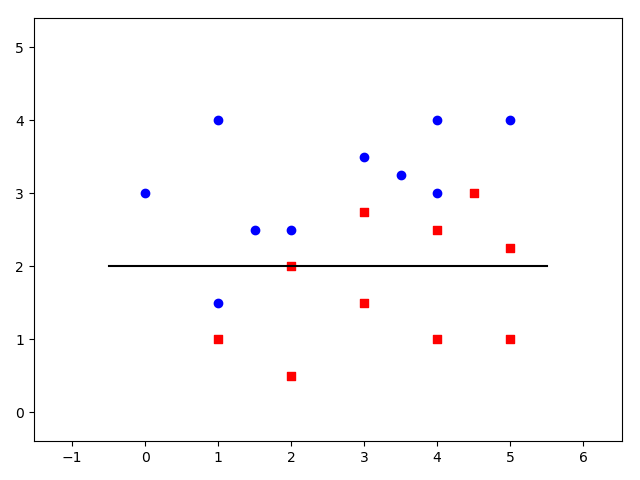
\includegraphics[scale=\myscale,scale=0.4]{figures/retro_01_b}
\end{minipage}
\begin{minipage}{0.45\textwidth}
\center \textbf{$k=1$ (première itération)}
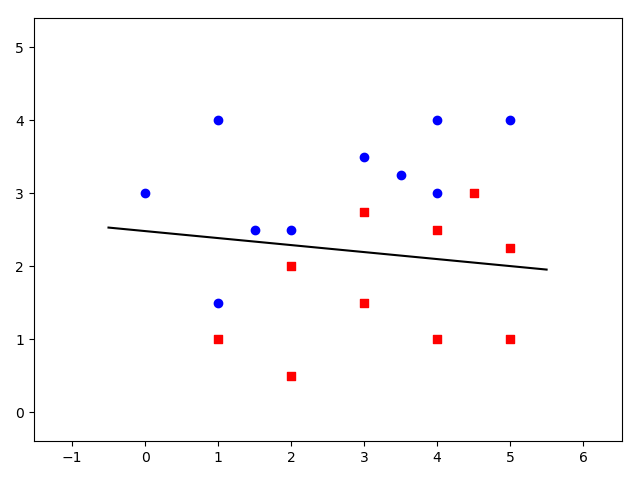
\includegraphics[scale=\myscale,scale=0.4]{figures/retro_01_c}
\end{minipage}

\begin{minipage}{0.45\textwidth}
\center \textbf{$k=100$}
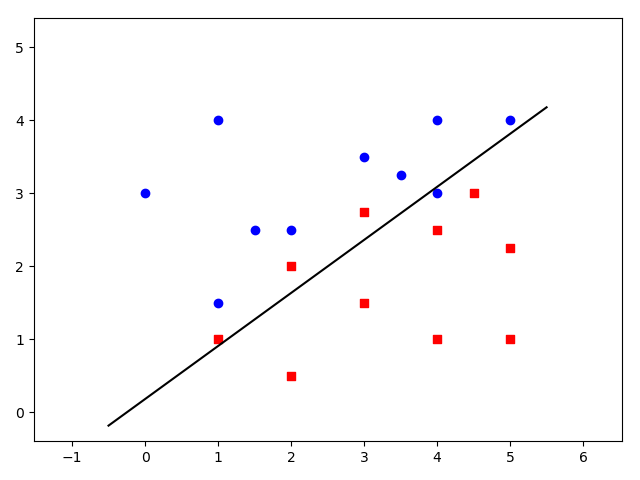
\includegraphics[scale=\myscale,scale=0.4]{figures/retro_01_d}
\end{minipage}
\begin{minipage}{0.45\textwidth}
\center \textbf{$k=1000$}
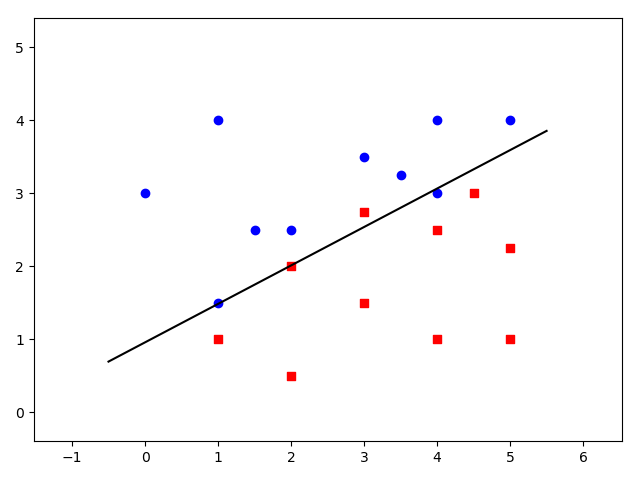
\includegraphics[scale=\myscale,scale=0.4]{figures/retro_01_e}
\end{minipage}
\end{center}

\end{itemize}  
\end{exemple}


%--------------------------------------------------------------------
\subsection{Prédiction}

La conception d'un réseau de neurones est réalisée en modélisant au mieux les données injectées. Mais l'objectif réel est de faire des prédictions pour de nouvelles valeurs, jamais rencontrées auparavant.
La descente de gradient produit un ensemble de poids $P$ qui définit complètement notre réseau $\mathcal{R}$.
Nous obtenons donc une fonction $F : \Rr^n \to \Rr$, construite de sorte que $F(X_i) \simeq z_i$.
Nous pouvons évaluer cette fonction pour tout $X \in \Rr^n$, même pour des $X$ différents des $X_i$.


\begin{exemple}
Dans notre exemple, nous avons obtenu par la descente de gradient les poids $P_{1000} = (a,b,c) = (2.032, -3.860, 3.703)$.
Notre neurone $\mathcal{R}$ est maintenant opérationnel et définit ici la fonction 
$$F(x,y) = \sigma(ax+by+c).$$

\begin{center}
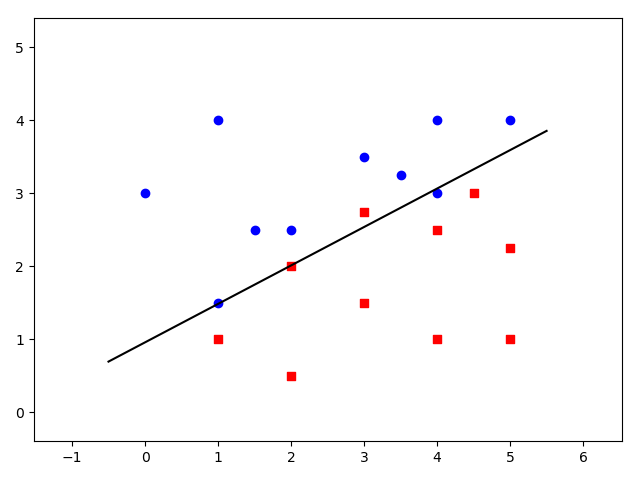
\includegraphics[scale=\myscale,scale=0.45]{figures/retro_01_e}
\end{center}

On souhaitait avoir $F(x_i,y_i)=0$ pour les ronds bleus et $F(x_i,y_i)=1$ pour les carrés rouges.
Dans la pratique, on obtient des valeurs approchées, par exemple $F(0,3)=0.0003$ pour le rond bleu en $(0,3)$ et $F(1,1)=0.86$ pour le carré rouge en $(1,1)$.

Notre fonction $F$ ne modélise pas parfaitement toutes nos données. Par exemple, pour le rond bleu en $(4,3)$ on a $F(4,3) = 0.56$ alors qu'on voudrait une valeur proche de $0$ et de même pour le carré rouge en $(3,2.75)$ on a $F(3,2.75) = 0.30$ alors qu'on voudrait une valeur proche de $1$. 

Mais l'intérêt principal de $F$ est d'être définie pour tous les points du plan, ceci permet d'attribuer une couleur à chaque point $(x,y) \in \Rr^2$ selon la convention : bleu si $F(x,y)\simeq 0$, rouge si $F(x,y) \simeq 1$. Il y a bien sûr une \og{}zone grise\fg{} entre les zones rouge et bleue.

Par exemple, $F(2,3) = 0.02$ donc $(2,3)$ mérite d'être colorié en bleu, $F(2,1) = 0.98$ donc $(2,1)$ mérite d'être colorié en rouge.
La frontière en laquelle $F$ vaut $\frac12$ est la droite d'équation $ax+by+c=0$.

Voici les niveaux de $F$ dans le plan (à gauche) et le graphe de $F$ dans l'espace (à droite).
\begin{center}
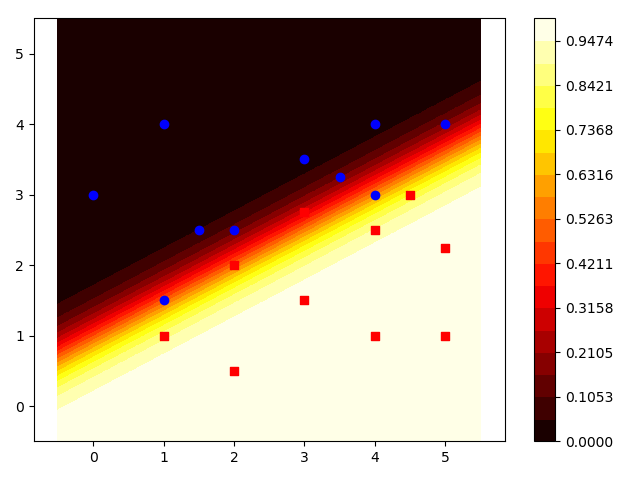
\includegraphics[scale=\myscale,scale=0.4]{figures/retro_01_g} \qquad
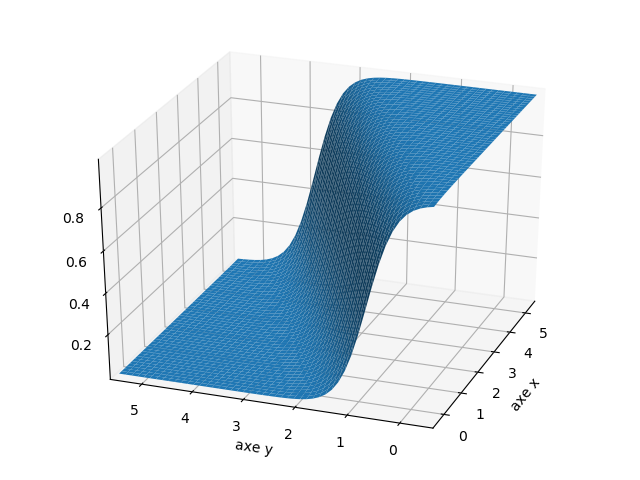
\includegraphics[scale=\myscale,scale=0.5]{figures/retro_01_f}
\end{center}


Nous avons choisi un réseau avec un seul neurone, la fonction $F$ est donc nécessairement très simple (quels que soient les poids) et ne peut pas \og{}coller\fg{} parfaitement aux données. 
Nous avons séparé au mieux les ronds bleus des carrés rouges par une droite. Avec un réseau plus complexe, et donc une frontière plus compliquée, nous aurions pu \og{}coller\fg{} parfaitement aux données. Cependant est-ce vraiment ce que nous souhaitons faire ? Pour les données de notre exemple, avoir une séparation par une droite semble raisonnable. Peut-être que les points transfuges sont des erreurs de mesure.

\end{exemple}




%%%%%%%%%%%%%%%%%%%%%%%%%%%%%%%%%%%%%%%%%%%%%%%%%%%%%%%%%%%%%%%%%%%%%
\section{Exemples}

%--------------------------------------------------------------------
\subsection{Le \og{}ou exclusif\fg{}}

Rappelons le problème du \og{}ou exclusif\fg{}\index{ou exclusif} : il s'agit de trouver un réseau de neurones dont la fonction associée $F$ vaut $1$ en $(0,1)$ et $(1,0)$ (les carrés rouges) et vaut $0$ en $(0,0)$ et $(1,1)$ (les rond bleus).

\myfigure{1}{
\tikzinput{fig_retro_01}
}

\textbf{Réseau.}

On a vu qu'il existe une solution avec un réseau à deux couches de fonction d'activation la fonction de Heaviside (voir le chapitre \og{}Réseau de neurones\fg{}).
On cherche à l'aide de la machine quels poids pourraient convenir avec la fonction d'activation sigmoïde :
\myfigure{1}{
\tikzinput{fig_retro_02}
}

Il y a donc $9$ coefficients à déterminer.
La fonction d'erreur est :
$$E = (F(0,0) - 0)^2 + (F(1,1) - 0)^2 + (F(0,1)-1)^2 + (F(1,0) - 1)^2$$
sachant que $F$ et donc l'erreur $E$ dépendent des coefficients $a_1,\ldots,a_9$.
Il s'agit de trouver ceux qui rendent l'erreur $E$ (presque) nulle.

\bigskip

\textbf{Descente de gradient.}
On applique la méthode de la descente de gradient à la fonction $E$ pour les variables $(a_1,\ldots,a_9)$.
On utilise la descente de gradient classique avec un pas $\delta = 1$. 
Le choix des poids initiaux est déterminant pour les résultats.
On choisit comme poids de départ :
$$P_0 = (a_1,\ldots,a_9) = (1.0, 2.0, -3.0, -3.0, -2.0, 1.0, 1.0, 1.0, -1.0).$$


L'erreur initiale vaut $E(P_0) = 0.2961$.
Le gradient $\grad E(P_0)$ vaut 
$$(0.00349, -0.00303, -0.00832, -0.00696, -0.01350, -0.01047, -0.00324, 0.01258, -0.04671).$$
Avec $\delta = 1$, la première itération modifie un petit peu les coefficients :
$$P_1 = (0.9965, 2.0030, -2.9916, -2.9930, -1.9864, 1.0104, 1.0032, 0.9874, -0.9532),$$
l'erreur a légèrement diminué et vaut maintenant $E(P_1) = 0.2935$.
La seconde itération donne :
$$P_2 = (0.9925, 2.0055, -2.9839, -2.9860, -1.9731, 1.0206, 1.0053, 0.9738, -0.9105)$$
et l'erreur vaut maintenant $E(P_2) = 0.2911$.

Au bout de $1000$ itérations :
$$P_{1000} = (3.5623, 3.5675, -5.5344, -5.3682, -5.3935, 1.8403, -6.3234, -6.3801, 3.1216)$$
et l'erreur vaut maintenant $E(P_{1000}) = 0.0097$.

\bigskip

\textbf{Validation et prédiction.}
Au bout de $1000$ itérations notre réseau de neurones est assez performant.
La fonction $F(x,y)$ obtenue vérifie :
$$F(0,0) = 0.08, \qquad F(1,1) = 0.10, \qquad F(1,0) = 0.89,  \qquad F(0,1) = 0.89.$$

Les ronds bleus sont donc clairement séparés des carrés rouges par les valeurs de $F$.

Quelle couleur est-il naturel d'associer au points $(0.2,0.9)$ ?
On calcule $F(0.2,0.9) = 0.87$ qui est assez proche de $1$, il est donc naturel de le colorier en rouge.

\bigskip

\textbf{Visualisation graphique.}
Voici deux représentations graphiques de la fonctions $F$ obtenue. À gauche par les lignes de niveau dans le plan et à droite par son graphe dans l'espace.
La fonction $F$ prend des valeurs proches de $1$ autour de la droite passant par $(1,0)$ et $(0,1)$
et se rapproche de $0$ partout ailleurs. 
\begin{center}
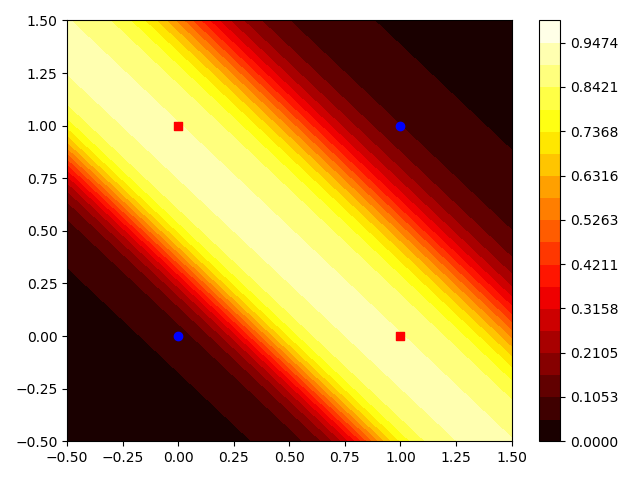
\includegraphics[scale=\myscale,scale=0.4]{figures/retro_02_a} \qquad
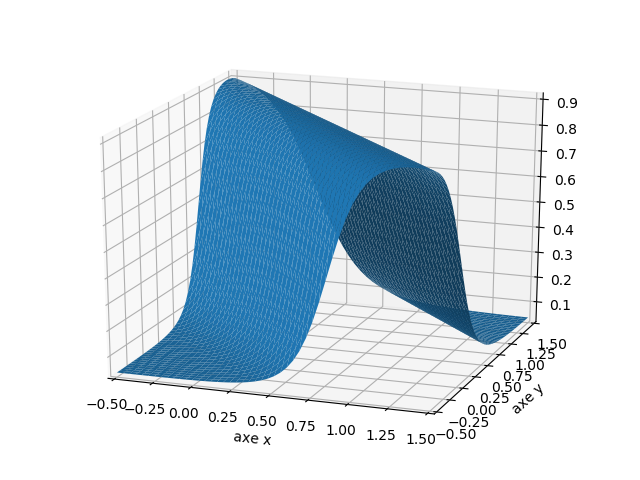
\includegraphics[scale=\myscale,scale=0.5]{figures/retro_02_b}
\end{center}

\bigskip

\textbf{Analyse.}
Voici l'évolution de l'erreur en fonction du nombre d'itérations. L'erreur décroît au fil des itérations : c'est le principe de la descente de gradient !
\begin{center}
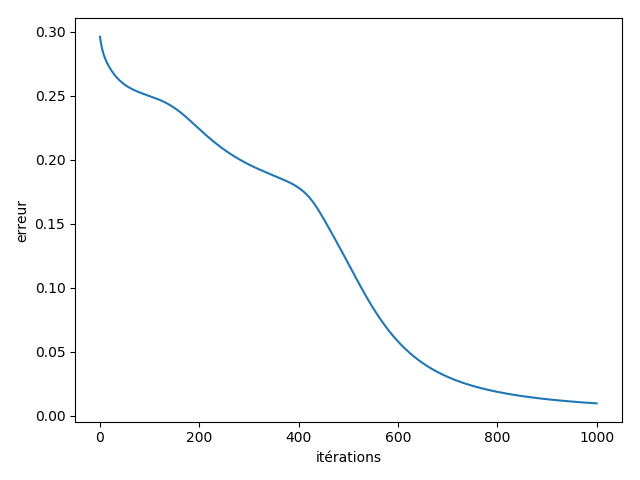
\includegraphics[scale=\myscale,scale=0.5]{figures/retro_02_c}
\end{center}


Comparer les poids obtenus avec ceux du \og{}ou exclusif\fg{} définis dans le chapitre \og{}Réseau de neurones\fg{}.

%--------------------------------------------------------------------
\subsection{Le perceptron et la règle de Hebb}

\index{perceptron}
\index{regle de Hebb@règle de Hebb}

Nous revenons sur l'exemple historique du cas d'un seul neurone (sans biais). Que donne la rétropropagation dans ce cas très simple ?

\myfigure{0.5}{
\tikzinput{fig_retro_08}
}

Nous souhaitons une fonction d'activation du type marche Heaviside, qui renvoie $0$ ou $1$, mais pour la descente du gradient nous avons besoin d'une dérivée non nulle. Nous allons imaginer qu'il existe une fonction marche de Heaviside virtuelle $\widetilde H$ telle que
$$\widetilde H(x) = 0 \quad \text{si $x <0$} \qquad \widetilde H(x)=1 \quad \text{si $x\ge0$} \quad \text{ et } \quad \widetilde H'(x) = 1 \quad \text{pour tout $x\in \Rr$}.$$
Il est clair qu'une telle fonction n'existe pas (car la dérivée d'une fonction constante par morceaux est toujours nulle) mais faisons comme si c'était le cas.

Ce neurone définit une fonction $F$ telle que $F(x_1,\ldots,x_n) = \widetilde H(a_1x_1+\cdots+a_nx_n)$.
Comme d'habitude, nous avons des données $(X_i,z_i)$, ici $z_i=0$ ou bien $z_i=1$. Il s'agit de trouver les poids 
$(a_1,\ldots,a_n)$ tels que $F(X_i) \simeq z_i$.
L'erreur locale est donnée par $E_i = \big( F(X_i) - z_i \big)^2$.

La descente de gradient (stochastique) pour la donnée $i$ s'écrit : 
$$P_{k+1} = P_k - \delta \grad E_i(P_k).$$
On a : 
$$\frac{\partial E_i}{\partial a_j}(X_i) = 2 \frac{\partial F}{\partial a_j}(X_i)  \big( F(X_i) - z_i \big).$$
Mais $\frac{\partial F}{\partial a_j}(X_i) = x_j$ car $\widetilde H'(x)=1$ et comme
$F(X_i)$ et $z_i$ valent $0$ ou $1$, alors 
$\frac{\partial E_i}{\partial a_j}(X_i)$ vaut $\pm 2x_j$ ou $0$. Autrement dit, 
$\grad E_i = 2\epsilon(x_1,\ldots,x_n) = 2\epsilon X_i$ avec $\epsilon = 0$, $1$ ou $-1$.

\bigskip

Nous avons ainsi obtenu la \defi{règle de Hebb}, qui est en fait l'ancêtre de la rétropropagation.

\textbf{Règle de Hebb.}
\begin{itemize}
  \item On fixe un pas $\delta>0$. 
  \item On part d'un poids $P_0$ (choisi au hasard par exemple).
  \item On calcule par récurrence les poids $P_k$ en parcourant la liste $(X_i,y_i)$ et en distinguant les cas suivants :
\begin{itemize}
  \item si la sortie prédite $F(X_i)$ vaut la sortie attendue $z_i$ alors on ne change rien :
  $$P_{k+1} = P_k,$$
  \item si la sortie prédite $F(X_i)$ vaut $1$ alors que la sortie attendue $z_i$ vaut $0$ alors :
    $$P_{k+1} = P_k - 2\delta X_i,$$
  \item si la sortie prédite $F(X_i)$ vaut $0$ alors que la sortie attendue $z_i$ vaut $1$ alors :
    $$P_{k+1} = P_k + 2\delta X_i.$$  
\end{itemize}

  \item Une fois toutes les données $(X_i,z_i)$ utilisées, on recommence depuis la première donnée.
  
  \item On s'arrête au bout d'un nombre d'itérations fixé à l'avance.
  \item Le dernier poids obtenu $P_k = (a_1,\ldots,a_n)$ définit le perceptron et la fonction associée qui répond au problème est :
  $F(x_1,\ldots,x_n)=1$ si $a_1x_1+\cdots+a_nx_n\ge0$ et $F(x_1,\ldots,x_n)=0$ sinon.
 
\end{itemize}



%--------------------------------------------------------------------
\subsection{Une fonction marche}

Nous avons vu dans le chapitre  \og{}Réseau de neurones\fg{} qu'il est facile de réaliser des fonctions \og{}marche\fg{} à l'aide d'un réseau simple et de la fonction de Heaviside.
Nous souhaitons construire un réseau de neurones dont la fonction $x \mapsto F(x)$ réalise au mieux les contraintes suivantes : $F(x)$ vaut $0$ sur $[0,2]$, puis vaut $1$ sur $[3,5]$ et de nouveau vaut
$0$ sur $[6,8]$ (il y a une certaine liberté sur $[2,3]$ et $[5,6]$).

\myfigure{0.7}{
\tikzinput{fig_retro_07}
}

\bigskip

\textbf{Données.}
On décide de placer $10$ ronds bleus espacés régulièrement sur $[0,2]$, la même chose sur 
$[6,8]$, là où la fonction doit être nulle, et également $10$ carrés rouges espacés régulièrement sur $[3,5]$ là où la fonction doit valoir $1$. Ces points fournissent donc les $N=30$ données d'apprentissage. 

\begin{center}
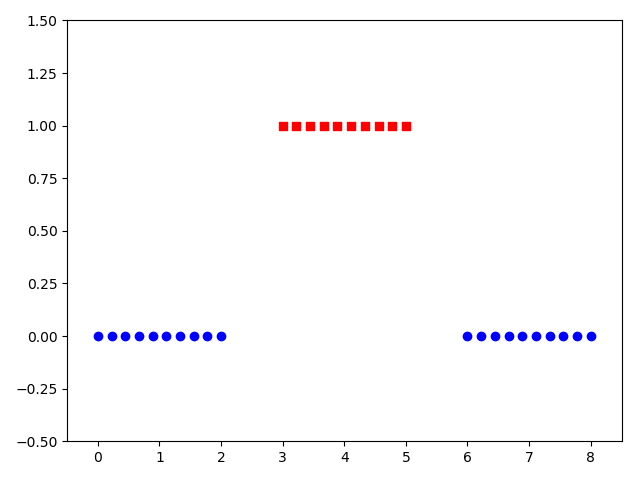
\includegraphics[scale=\myscale,scale=0.4]{figures/retro_03_a}
\end{center}

\bigskip

\textbf{Réseau.}
On décide d'utiliser un réseau avec deux neurones sur la couche d'entrée et un neurone sur la couche de sortie, tous utilisant la fonction d'activation $\sigma$.

\myfigure{1}{
\tikzinput{fig_retro_09}
}

Il y a $7$ coefficients à déterminer.
La fonction d'erreur $E$ est la somme des $(F(x_i)-0)^2$ pour les $x_i$ abscisses des ronds bleus et des $(F(x_i)-1)^2$ pour les $x_i$ abscisses des carrés rouges.

\bigskip

\textbf{Descente de gradient.}
On applique la descente de gradient à la fonction $E$ de variables $(a_1,\ldots,a_7)$ pour un pas $\delta = 1$ et un choix arbitraire de poids initiaux :
$$P_0 = (a_1,\ldots,a_7) = (0.0, 1.0, 0.0, -1.0, 1.0, 1.0, -1.0).$$

Au bout de $5000$ itérations, on obtient les poids :
$$P_{5000} = (a_1,\ldots,a_7) = (-2.0142, 10.9964, 3.0543, -7.7086, 8.2334, 7.8735, -11.9037).$$


Voici l'évolution de l'erreur en fonction du nombre d'itérations.
 \begin{center}
 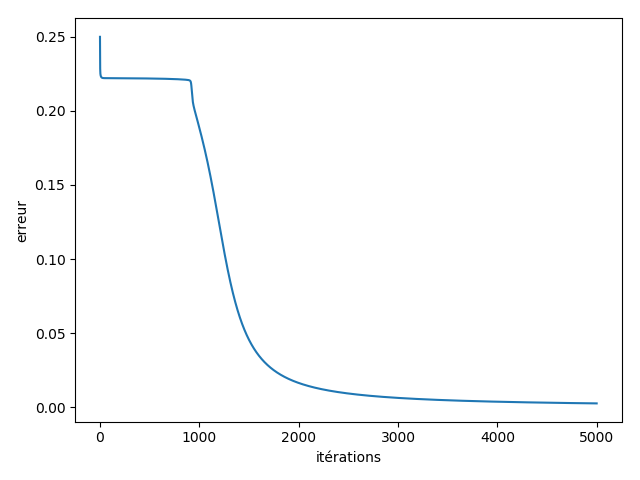
\includegraphics[scale=\myscale,scale=0.5]{figures/retro_03_f}
 \end{center}
 
 
\bigskip

\textbf{Visualisation graphique.}

Voici le graphe de la fonction $x \mapsto F(x)$ au bout de différents nombres d'itérations.

\begin{center}
\begin{minipage}{0.45\textwidth}
\center \textbf{$k=0$ (initialisation)} 
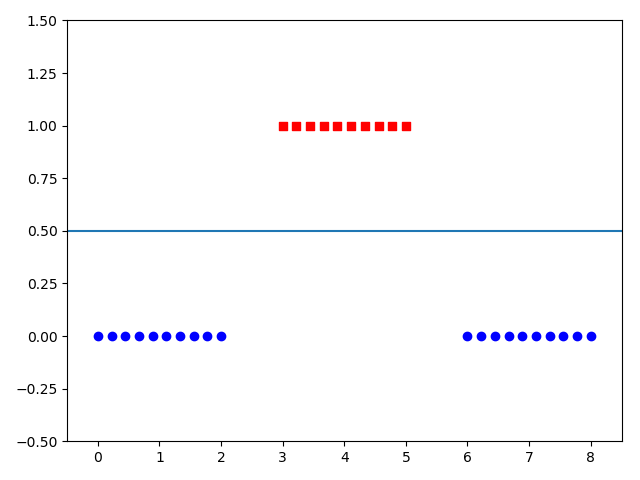
\includegraphics[scale=\myscale,scale=0.45]{figures/retro_03_b}
\end{minipage}
\begin{minipage}{0.45\textwidth}
\center \textbf{$k=1000$}
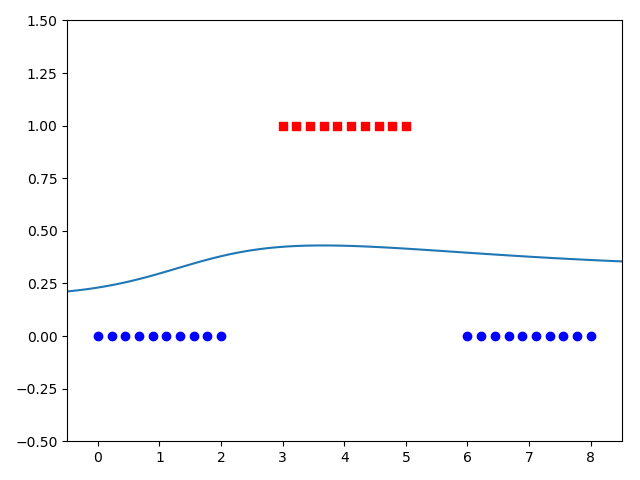
\includegraphics[scale=\myscale,scale=0.45]{figures/retro_03_c}
\end{minipage}

\begin{minipage}{0.45\textwidth}
\center \textbf{$k=2000$}
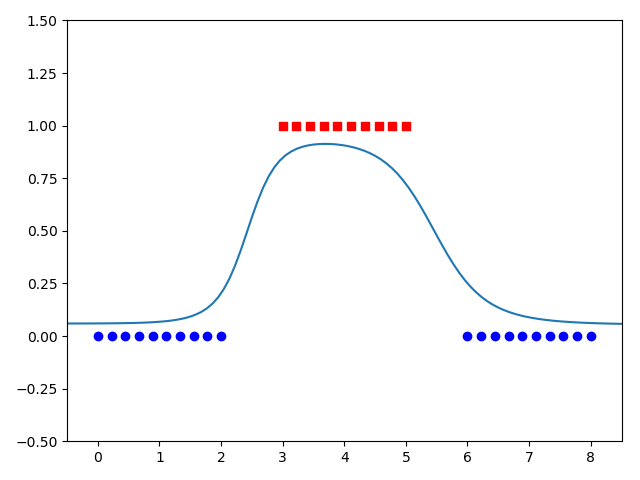
\includegraphics[scale=\myscale,scale=0.45]{figures/retro_03_d}
\end{minipage}
\begin{minipage}{0.45\textwidth}
\center \textbf{$k=5000$}
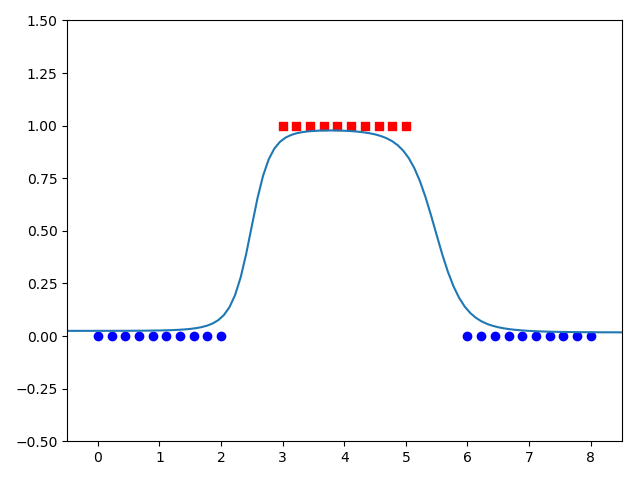
\includegraphics[scale=\myscale,scale=0.45]{figures/retro_03_e}
\end{minipage}
\end{center}


%--------------------------------------------------------------------
\subsection{Plus de neurones}

Le but est de trouver un réseau de neurones qui distingue deux zones compliquées du plan : la zone bleue et la zone rouge.

\myfigure{1}{
\tikzinput{fig_retro_10d}
}



Voici comme sont construites ces zones : on part d'une lemniscate de Bernoulli d'équation $(x^2+y^2)^2 = 4(x^2-y^2)$ et d'une ellipse d'équation
$(x-\frac12)^2 + 4(y-\frac13)^2=2$. 

\begin{center}
\begin{minipage}{0.31\textwidth}
\myfigure{0.47}{
\tikzinput{fig_retro_10a}
}
\end{minipage}
\quad
\begin{minipage}{0.31\textwidth}
\myfigure{0.47}{
\tikzinput{fig_retro_10b}
}

\end{minipage}
\quad
\begin{minipage}{0.31\textwidth}
\myfigure{0.47}{
\tikzinput{fig_retro_10c}
}
\end{minipage}
\end{center}


L'union de ces deux courbes a pour équation :
$$f(x,y) = \big( (x^2+y^2)^2 - 4(x^2-y^2) \big)  \cdot \big((x-\tfrac12)^2 + 4(y-\tfrac13)^2 - 2 \big) = 0.$$
La zone rouge correspond aux points de coordonnées $(x,y)$ pour lesquels $f(x,y) \le 0$ et la zone bleue à $f(x,y) > 0$. Nous allons limiter notre étude à une zone rectangulaire. Le rectangle est choisi de sorte que l'aire bleue et l'aire rouge soient à peu près égales.

\textbf{Objectifs.} 
On oublie maintenant la fonction $f$ et on ne retient que quelques points rouges et quelques points bleus. On cherche un réseau et une fonction $F$ telle que $F(x,y) \simeq 1$ pour les points rouges et $F(x,y) \simeq 0$ pour les points bleus.

\textbf{Données.} 
On divise notre rectangle en une grille de $n \times n$ points. Les exemples ci-dessous sont calculés pour $n=200$. Nous avons donc $40\,000$ points $(x,y)$, repartis (à peu près) équitablement entre rouge ($z=1$) et bleu ($z=0$).

\textbf{Architecture.}
On décide de concevoir un réseau à $4$ couches, avec le même nombre $p$ de neurones par couche pour les trois premières couches et un seul neurone sur la couche de sortie. La fonction d'activation choisie pour tous les neurones est ReLU .
Voici une illustration de la configuration pour $p=3$.

\myfigure{0.8}{
\tikzinput{fig_retro_11}
}


\textbf{Poids.} 
On calcule les poids avec une méthode de descente de gradient stochastique.
Les poids initiaux sont choisis aléatoirement, le nombre d'itérations est suffisamment grand.
Le réseau obtenu après calculs fournit donc une fonction $F$.
On colorie en rouge les points pour lesquels $F(x,y) \simeq 1$ (en fait, là où $F(x,y)\ge \frac12$) et en bleu les points pour lesquels $F(x,y) \simeq 0$ (en fait, là où $F(x,y)< \frac12$). On regarde si le résultat obtenu est proche de la situation envisagée.
On présente ici quelques résultats typiques intéressants (les résultats pouvant varier selon le choix aléatoire des poids initiaux).

\begin{center}
\begin{minipage}{0.45\textwidth}
\center {$p=3$, $10$ neurones, $37$ poids} 
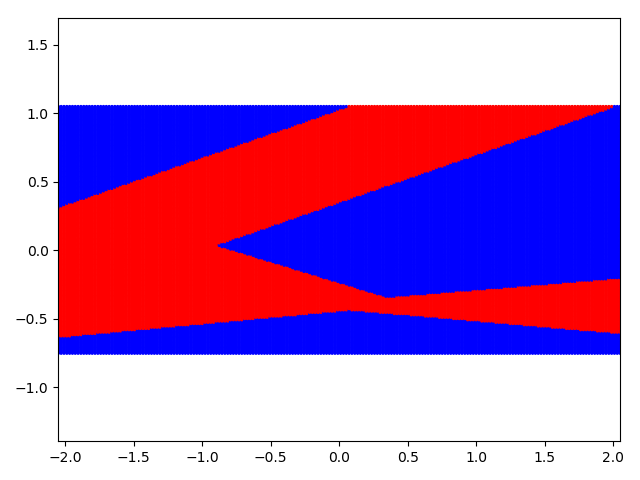
\includegraphics[scale=\myscale,scale=0.45]{figures/retro_05_p=3}
\end{minipage}
\begin{minipage}{0.45\textwidth}
\center {$p=5$, $16$ neurones, $81$ poids}
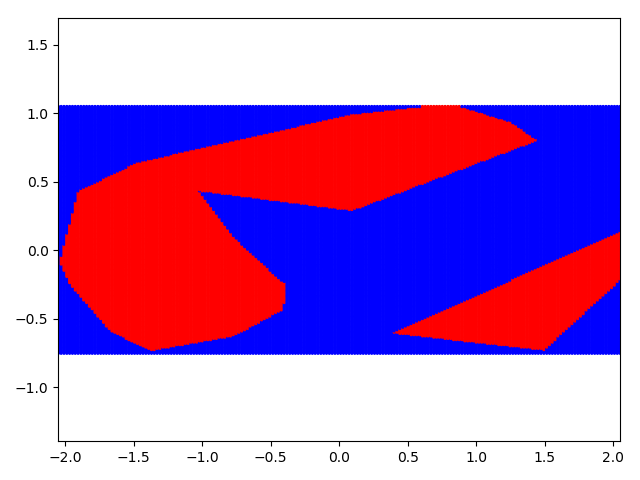
\includegraphics[scale=\myscale,scale=0.45]{figures/retro_05_p=5}
\end{minipage}
\end{center}


\begin{center}
\begin{minipage}{0.45\textwidth}
\center {$p=7$, $22$ neurones, $141$ poids} 
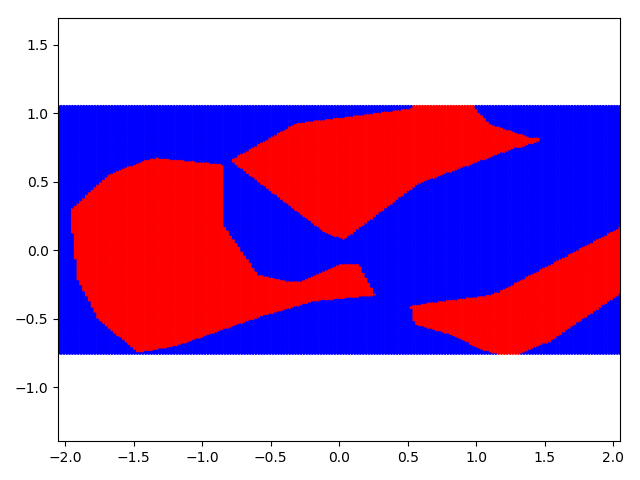
\includegraphics[scale=\myscale,scale=0.45]{figures/retro_05_p=7}
\end{minipage}
\begin{minipage}{0.45\textwidth}
\center {$p=10$, $31$ neurones, $261$ poids}
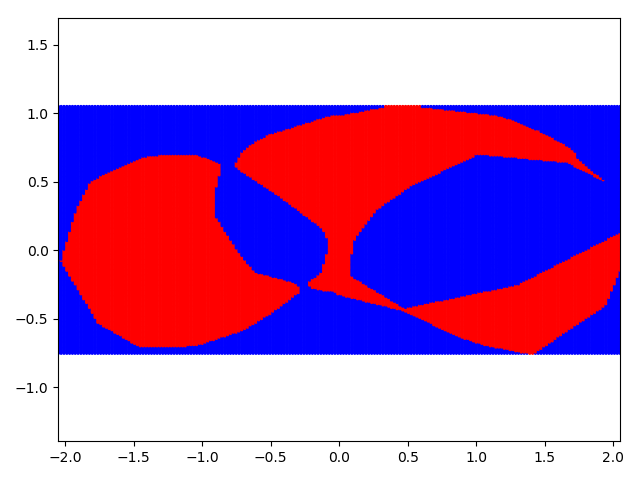
\includegraphics[scale=\myscale,scale=0.45]{figures/retro_05_p=10}
\end{minipage}
\end{center}


\begin{center}
\begin{minipage}{0.45\textwidth}
\center {$p=15$, $46$ neurones, $541$ poids} 
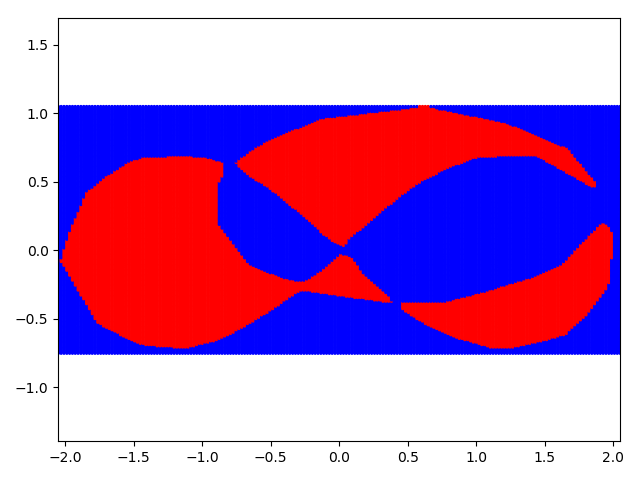
\includegraphics[scale=\myscale,scale=0.45]{figures/retro_05_p=15}
\end{minipage}
\begin{minipage}{0.45\textwidth}
\center {$p=20$, $61$ neurones, $921$ poids}
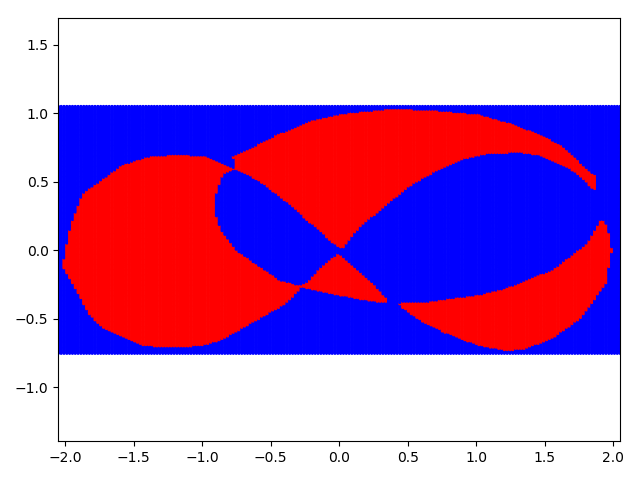
\includegraphics[scale=\myscale,scale=0.45]{figures/retro_05_p=20}
\end{minipage}
\end{center}

\begin{center}
\begin{minipage}{0.45\textwidth}
\center {$p=50$, $151$ neurones, $5301$ poids} 
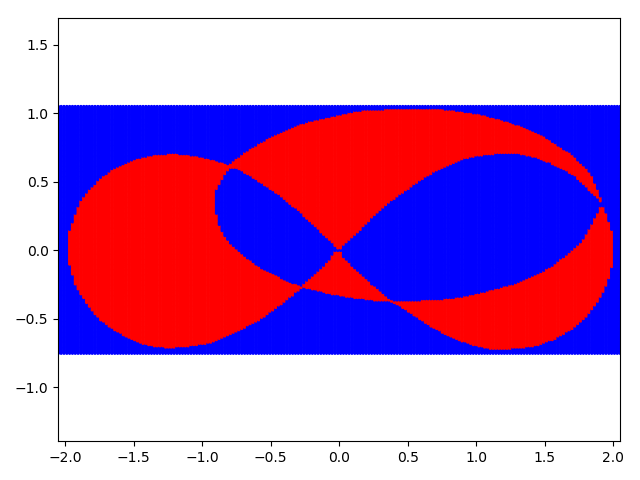
\includegraphics[scale=\myscale,scale=0.45]{figures/retro_05_p=50}
\end{minipage}
\begin{minipage}{0.45\textwidth}
\center {$p=100$, $301$ neurones, $20\,601$ poids}
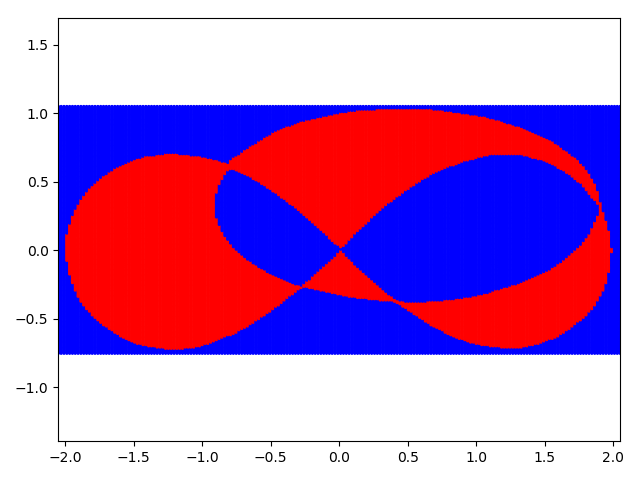
\includegraphics[scale=\myscale,scale=0.45]{figures/retro_05_p=100}
\end{minipage}
\end{center}


Conclusion : il faut un nombre assez grand de neurones pour pouvoir modéliser des phénomènes compliqués. Dans l'exemple traité ici, on obtient une bonne approximation à partir de $p=20$, soit plus de $60$ neurones et environ $1000$ poids.

 
%--------------------------------------------------------------------
\subsection{Apprentissage}

N'oublions pas le but principal des réseaux de neurones : apprendre à partir des données afin de prédire des résultats pour des situations nouvelles.


Voici un problème pour lequel nous allons tester si les prédictions sur des données nouvelles sont correctes ou pas.
On dispose de $n$ cases, dont $3$ sont noircies.  On appelle \emph{hauteur}, le nombre total de cases entre la plus haute et la plus basse case noircie. Si les trois cases ont pour rang $i < j <k$ alors la hauteur vaut $h = k-i+1$ (la case noircie du milieu n'intervient pas dans la formule).
Sur le dessin ci-dessous, $n=8$ et la configuration représentée est de hauteur $6$.

\myfigure{1}{
\tikzinput{fig_retro_12}
}

Il y a en tout $N = \frac{n(n-1)(n-2)}{6}$ configurations possibles pour les trois cases noires parmi $n$ cases.
On décide d'utiliser la moitié des configurations comme données d'apprentissage et l'autre moitié va nous permettre de tester si le réseau calculé avec les données d'apprentissage se comporte \og{} correctement\fg{} sur les nouvelles données.

Dans la suite nous prendrons $n=20$ cases, ce qui fait $N=1140$ configurations possibles.

\textbf{Données en entrées.}
On calcule les $N$ configurations possibles. Après un mélange aléatoire, on ne retient que $N/2$ configurations pour l'apprentissage. Une configuration est codée sous la forme d'un vecteur
$X = (x_1,x_2,\ldots,x_n)$ avec $x_i=0$ (case blanche) ou $x_i = 1$ (case noire).
Pour chaque configuration $X$ des données d'apprentissage, on calcule la hauteur $z = h(X)$. Les données d'apprentissage sont les $N/2$ données $(X_k,z_k)$ formées des entrées $X_k$ et de la sortie attendue $z_k$ (la hauteur). 

\textbf{Réseau.}
Le réseau comporte $n$ entrées : une entrée par case. Il est constituée de $3$ couches.
Les deux premières couches possèdent $p$ neurones et la couche de sortie un seul. La fonction d'activation est la fonction ReLU pour tous les neurones. Sur la figure ci-dessous est illustré le cas $p=5$.

\myfigure{1}{
\tikzinput{fig_retro_13}
}


\textbf{Apprentissage.}
Le réseau est initialisé avec des poids aléatoires. Ensuite ces poids sont modifiés par une descente de gradient stochastique avec un nombre suffisant d'itérations.

\textbf{Sortie prédite.}
Le réseau paramétré fournit une fonction $F$ à valeur réelle. La sortie attendue étant un entier, on décide que la sortie prédite sera arrondie à l'entier le plus proche.
Pour chaque $X_k$, la prédiction est correcte si la valeur arrondie $F(X_k)$ vaut la hauteur $h(X_k)$. 


\textbf{Tests.}
Il faut tester l'efficacité du réseau : tout d'abord le réseau modélise-t-il correctement les données d'apprentissage ? En effet, même si la fonction $F$ a été construite dans le but d'avoir $F(X_k) \simeq z_k$, il n'y a pas nécessairement égalité pour toutes les données d'apprentissage. Mais surtout, il faut tester si la fonction $F$ donne de bonnes prédictions pour de nouvelles données. Nous disposons pour cela des $N/2$ données de test non utilisées lors de l'apprentissage.

Les résultats dépendent des poids initiaux (aléatoires) et de la liste des configurations (qui a été mélangée), on ne retient que les meilleurs résultats parmi plusieurs essais.
Par exemple, pour $p=10$, voici un des meilleurs résultats obtenus :
\begin{itemize}
  \item \emph{Apprentissage.} $560$ données prédites correctement sur un total de de $570$ données d'apprentissage, soit $98\%$ de réussite.
  
  \item \emph{Test.} $506$ données prédites correctement sur un total de de $570$ données de test, soit $89\%$ de réussite.
\end{itemize}

Voici quelques résultats pour différentes valeurs de $p$.

\begin{center}
\begin{tabular}{c|c|c|c|c}
$p$ & {neurones} & {poids} & {pourcentage apprentissage} & {pourcentage test} \\ \hline
3 & 7 & 79 & 50\% & 45\% \\
5 & 11 & 141 & 85\% & 75\% \\
7 & 15 & 211 & 90\% & 85\% \\
10 & 21 & 331 & 98\% & 90\% \\
15 & 36 & 571 & 99\% & 90\% \\
20 & 41 & 861 & 100\% & 85\% \\
\end{tabular}
\end{center}

\textbf{Commentaires.} Plus il y a de neurones, plus la fonction $F$ modélise correctement les données d'apprentissage : à partir de $20$ neurones ($p\ge10$), la modélisation est quasi-parfaite. Les pourcentages de réussite pour les données de test sont toujours inférieures et plafonnent à 90\%. Un phénomène nouveau apparaît avec plus de $40$ neurones (pour $p=20$), les pourcentages de réussite sur les tests régressent par rapport à des réseaux ayant moins de neurones, bien que les données d'apprentissage soient parfaitement modélisées : c'est un phénomène de sur-apprentissage.



%%%%%%%%%%%%%%%%%%%%%%%%%%%%%%%%%%%%%%%%%%%%%%%%%%%%%%%%%%%%%%%%%%%%%
\section{Sur-apprentissage et autres soucis}

Nous allons voir différents problèmes qui peuvent intervenir dans le calcul des poids d'un réseau de neurones, le problème le plus subtil étant le \emph{sur-apprentissage}. 


%--------------------------------------------------------------------
\subsection{Modèle insuffisant}

\textbf{Problème.}
Voici deux exemples de situations dans lesquelles le choix de l'architecture du réseau pose problème, car le réseau est trop simple. 

\bigskip

\textbf{Exemple 1.}
Imaginons que nous voulions modéliser une situation à partir des données fournies par les points $(x_i,y_i)$ du plan (figure de gauche). Si on construit un réseau d'un seul neurone (figure de droite), alors la fonction de sortie sera du type $y= F(x) = ax+b$.
\begin{center}
\begin{minipage}{0.45\textwidth}
\myfigure{0.7}{
\tikzinput{fig_soucis_02}
}
\end{minipage}
\begin{minipage}{0.45\textwidth}
\myfigure{1}{
\tikzinput{fig_soucis_01}
}
\end{minipage}
\end{center}

Aucun paramètre $(a,b)$ ne permettra une modélisation correcte de la situation, car les points ne sont franchement pas alignés.

\bigskip

\textbf{Exemple 2.}
Le même problème se produirait si on voulait trouver une fonction $F$, construite à partir d'un seul neurone, valant $0$ pour la zone bleue et $1$ pour la zone rouge de la figure ci-dessous. Ce n'est pas possible car la frontière de la solution n'est pas linéaire.

\begin{center}
\begin{minipage}{0.45\textwidth}
\myfigure{1}{
\tikzinput{fig_soucis_03}
}
\end{minipage}
\begin{minipage}{0.45\textwidth}
\myfigure{0.7}{
\tikzinput{fig_soucis_04}
}
\end{minipage}
\end{center}

\bigskip

\textbf{Conclusion.} Dans ces situations, le problème ne se situe pas au niveau des poids, augmenter la taille des données ou le nombre d'itérations n'y changera rien. La conception du réseau est mauvaise pour répondre à la question posée. C'est comme vouloir faire une course de voitures avec une deux-chevaux. La solution est de changer l'architecture du réseau, par exemple en rajoutant des neurones.

%--------------------------------------------------------------------
\subsection{Minimum local}

\index{minimum!local}

\textbf{Problème.} La descente de gradient a pour objectif de fournir un minimum local. 
Cependant rien n'affirme que ce minimum local est un minimum global.

\bigskip

\textbf{Exemple.}
Voici un réseau composé d'un seul neurone de fonction d'activation ReLU et possédant un seul coefficient à déterminer, le biais étant imposé à la valeur $-1$.
\myfigure{0.7}{
\tikzinput{fig_soucis_08}
}
Le graphe de la fonction $F$ correspondant à ce neurone est une portion de la droite d'équation $y=ax-1$, prolongée par l'axe des abscisses. Voici l'exemple du graphe de $F$, avec $a=+2$. 

\begin{center}
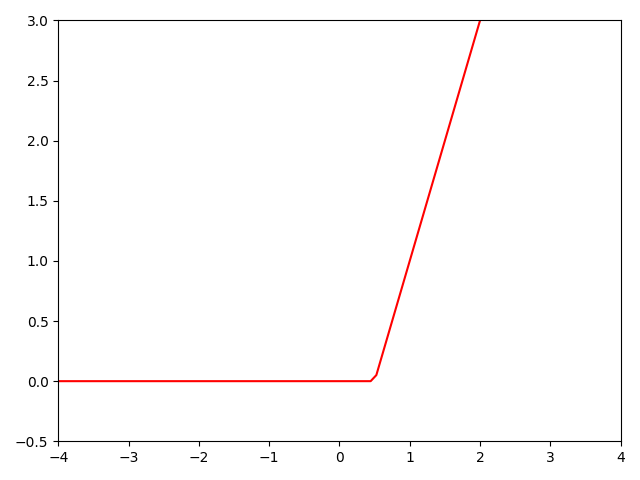
\includegraphics[scale=\myscale,scale=0.45]{figures/retro_04_d}
\end{center}

Les données sont des points déterminés par leurs coordonnées $(x_i,y_i)$ :
$$(-2,1),\quad  (-1,0),\quad (0,0),\quad (1,0),\quad (3,2).$$

\begin{center}
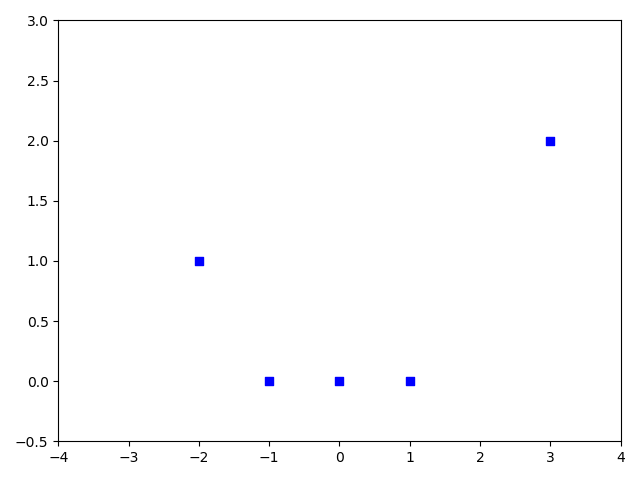
\includegraphics[scale=\myscale,scale=0.45]{figures/retro_04_a}
\end{center}

Il s'agit de trouver le meilleur coefficient $a$, qui définisse $F$ tel que $F(x_i) \simeq y_i$. Autrement dit, on souhaite minimiser $E(a) = \sum E_i(a)$ où $E_i(a) = (F(x_i)-y_i)^2$.
Géométriquement il y a deux paramètres qui semblent meilleurs que les autres $a=-1$ (figure de gauche) et $a=+1$ (figure de droite) car alors les portions de droites passent par des carrés\couleurnb{ bleus}{}.

\begin{center}
\begin{minipage}{0.45\textwidth}
\center \textbf{$a=-1$}
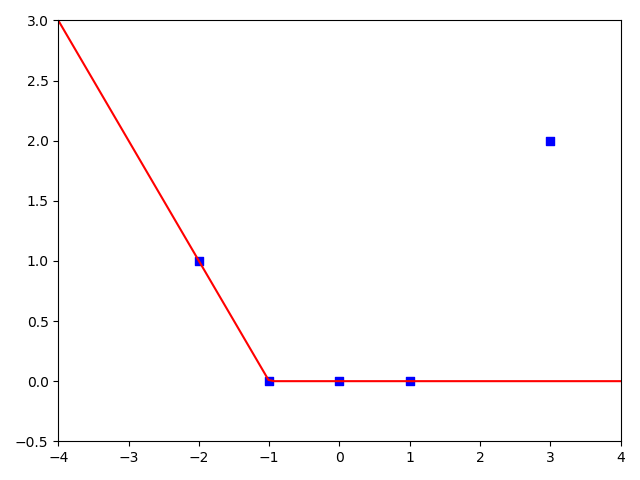
\includegraphics[scale=\myscale,scale=0.45]{figures/retro_04_b}
\end{minipage}
\begin{minipage}{0.45\textwidth}
\center \textbf{$a=+1$}
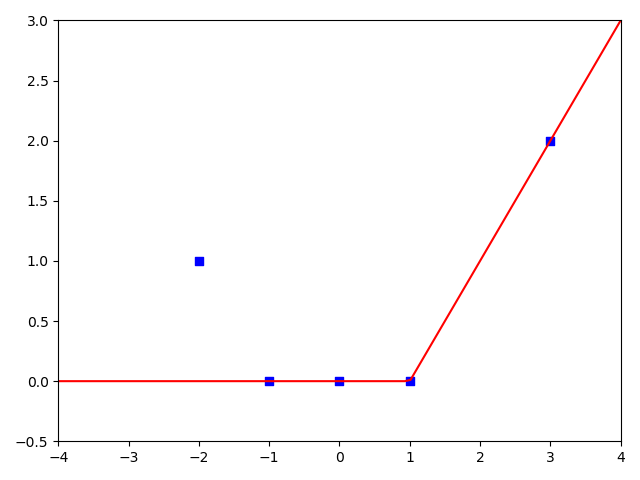
\includegraphics[scale=\myscale,scale=0.45]{figures/retro_04_c}
\end{minipage}
\end{center}

Cette intuition se vérifie lorsque l'on trace le graphe de la fonction d'erreur $a \mapsto E(a)$. La fonction possède deux minimums locaux en $a=-1$ et $a=+1$ (et aussi une portion constante, due à l'usage de la fonction ReLU).
\begin{center}
\textbf{Erreur $E(a)$ en fonction du coefficient $a$}

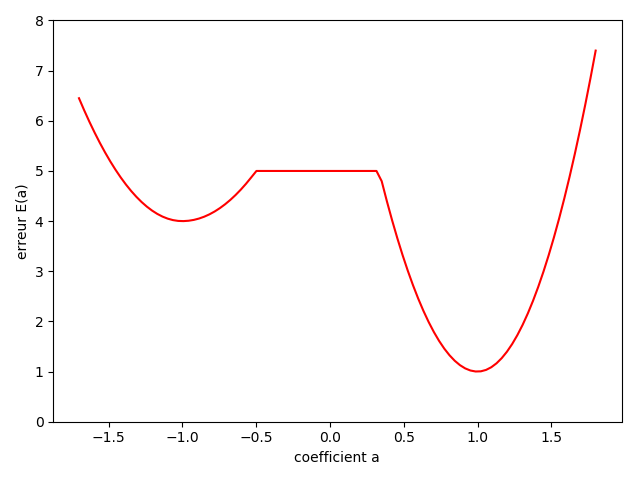
\includegraphics[scale=\myscale,scale=0.45]{figures/retro_04_e}
\end{center}
Le minimum en $a=+1$ est le minimum global. Mais si on applique la descente de gradient en partant d'un coefficient initial $a_0<0$, il y a de grandes chances d'arriver au minimum local $a=-1$, qui ne sera pas la solution optimale.

\bigskip

\textbf{Conclusion.} Vous êtes une fourmi qui se promène dans une boîte d'\oe ufs avec des trous de différentes profondeurs : vous ne pouvez pas voir à l'avance quel est l'emplacement le plus profond ! Une solution peut être de tester différentes valeurs initiales, dans le but d'obtenir différents minimums locaux.

%--------------------------------------------------------------------
\subsection{Sous-apprentissage}

\textbf{Problème.}
Le \defi{sous-apprentissage} révèle une conception correcte de l'architecture du réseau mais une mauvaise mise en \oe uvre. On obtient alors des poids qui ne répondent pas correctement au problème.

\bigskip
\textbf{Exemple.} Une droite obtenue par un réseau approche mal une suite de points pourtant alignés.
\myfigure{0.7}{
\tikzinput{fig_soucis_05}
}

Cela peut être dû aux raisons suivantes :
\begin{itemize}
  \item les données ne sont pas en nombre suffisant, 
  \item le nombre d'itérations est insuffisant,
  \item le pas $\delta$ est trop grand.
\end{itemize}

\bigskip

\textbf{Conclusion.} 
Il est difficile de savoir à l'avance quelle est la bonne taille
des données à utiliser et combien d'itérations sont nécessaires pour arriver à un modèle correct. Le sous-apprentissage, c'est comme faire une course de voiture avec une porsche mais en ne dépassant jamais les 80 km/h !
A posteriori, la solution est simple : ajouter des données, augmenter le nombre d'itérations ou diminuer la pas.

 
%--------------------------------------------------------------------
\subsection{Sur-apprentissage}

\index{sur-apprentissage}

\textbf{Problème.} Le modèle obtenu \og{}colle\fg{} parfaitement aux données d'apprentissage, mais cependant les prédictions pour de nouvelles valeurs sont mauvaises.
Il s'agit donc d'un problème délicat : la fonction $F$ obtenue vérifie bien $F(X_i) \simeq z_i$ pour toutes les données, mais pour une nouvelle entrée $X$, la sortie $F(X)$ n'est pas une bonne prédiction. Cela se produit lorsque l'on se concentre uniquement sur l'apprentissage à partir des données, mais que l'on a oublié que le but principal est la prédiction.

\bigskip

% Les exemples qui suivent ne sont pas vraiment issue de réseau de neurone, mais d'interpolation polynomiale, ce qui est plus parlant.

\textbf{Exemple 1.} Nous avons $4$ points\couleurnb{ bleus}{}.
Pour une valeur $x_0$ donnée, on souhaite prédire une valeur $y_0$ (figure de gauche) cohérente avec nos données.

On propose dans un premier temps d'approcher la solution en utilisant une droite (figure de droite) même si les points ne sont pas exactement alignés. Cela permet de prédire une valeur $y_0$ pour placer le point $P=(x_0,y_0)$.
Ce modèle ne sera jamais parfait car les points ne sont pas alignés, donc aucune droite ne convient exactement, autrement dit l'erreur ne sera jamais nulle.

\myfigure{0.7}{
\tikzinput{fig_soucis_06a}
\tikzinput{fig_soucis_06b}
}

On peut construire un modèle plus compliqué, par exemple chercher une courbe polynomiale de degré $3$ ou plus qui passe \emph{exactement} par tous les points d'apprentissage. Ainsi, pour cette courbe, l'erreur sera nulle. Cette courbe permet de prédire une valeur $y_0'$ pour placer un point $P'(x_0,y_0')$. 

\myfigure{0.8}{
\tikzinput{fig_soucis_06c}
}
Ce dernier modèle répond entièrement au problème, mais la solution proposée ne semble pas raisonnable par rapport aux données de départ. C'est un cas de sur-apprentissage : le modèle est correct sur les données, mais les prédictions seront mauvaises.

\bigskip

\textbf{Exemple 2.}
Le problème est similaire si on essaye de séparer les ronds bleus des carrés rouges de la figure de gauche ci-dessous. Une modèle simple permet à une parabole de séparer l'essentiel des ronds bleus des carrés rouges (figure centrale). On peut entraîner un modèle plus complexe pour qu'il délimite parfaitement les deux types de points, mais au prix d'une complexité non nécessairement voulue (figure de droite).
\myfigure{0.7}{
\tikzinput{fig_soucis_07a}\qquad
\tikzinput{fig_soucis_07b}\qquad
\tikzinput{fig_soucis_07c}
}

\textbf{Conclusion.}
Le sur-apprentissage, c'est comme emmener ses enfants à l'école en conduisant à 200 km/h : cela répond de façon correcte à un problème, mais cela provoque beaucoup d'autres ennuis !  
Quelle est la meilleure solution entre un modèle simple mais imparfait et un modèle parfait mais compliqué ? Il n'y a pas une réponse immédiate à la question : pour savoir, il faut tester le modèle sur d'autres données, jamais rencontrées, afin de déterminer si le réseau n'a pas été sur-entraîné.


\end{document}
